\documentclass[11pt]{article}
\usepackage{amsmath}
\usepackage{geometry}
\geometry{margin=1in}
\usepackage{graphicx}
\usepackage{amssymb}
\usepackage{float} % Required for the [H] figure placement specifier

\title{\textbf{CS589: Homework 2}}
\author{Vishnu Vardhan Reddy B.}
\date{September 24, 2025}

\begin{document}
\maketitle

\section*{Question 1: Generalization and Model Capacity}
\noindent\textbf{(a)} The OOD (out-of-distribution) problem is what happens when we train a model on data from one distribution (P) but then deploy it on data from a different one (Q). If we only estimate performance on a test set from P, we can get a misleading idea of how the model will perform in the real world, since P and Q are different. This "distribution shift" is the main challenge of the OOD problem.

\noindent\textbf{(b)} When the training error is a lot lower than the test error, it's a clear sign the model is overfitting. This means it has essentially memorized the training data, including its noise, and as a result, it can't generalize well to new, unseen data. This usually happens when the model's capacity is too high for the dataset. A good way to combat this is with regularization, which adds a penalty to the loss function to discourage the model from becoming too complex, helping it perform better.
\section*{Question 2: Learning Probability Mass Functions}
\noindent\textbf{(a)} We show that $P(X=x_{n})=\pi_{0}^{\mathbb{I}(x_{n}=0)}\cdot\pi_{1}^{\mathbb{I}(x_{n}=1)}$ reduces to $P(X=x_{n})=\pi_{x_{n}}$ for $x_n \in \{0, 1\}$.  
\begin{itemize}
    \item Case $x_n = 0$: $P(X=0) = \pi_{0}^{1} \cdot \pi_{1}^{0} = \pi_0$.
    \item Case $x_n = 1$: $P(X=1) = \pi_{0}^{0} \cdot \pi_{1}^{1} = \pi_1$.
\end{itemize}

\noindent\textbf{(b)} Starting with $nall(\pi, \mathcal{D}) = -\frac{1}{N_{tr}}\sum_{n=1}^{N_{tr}}\log P(X=x_{n})$ and substituting the PMF:
\begin{align*}
    nall(\pi, \mathcal{D}) &= -\frac{1}{N_{tr}}\sum_{n=1}^{N_{tr}}\log \left( \pi_{0}^{\mathbb{I}(x_{n}=0)}\cdot\pi_{1}^{\mathbb{I}(x_{n}=1)} \right) \\
    &= -\frac{1}{N_{tr}}\sum_{n=1}^{N_{tr}} \left[ \log\left(\pi_{0}^{\mathbb{I}(x_{n}=0)}\right) + \log\left(\pi_{1}^{\mathbb{I}(x_{n}=1)}\right) \right] \\
    &= -\frac{1}{N_{tr}}\sum_{n=1}^{N_{tr}} \left[ \mathbb{I}(x_{n}=0)\log(\pi_{0}) + \mathbb{I}(x_{n}=1)\log(\pi_{1}) \right] \\
    &= -\frac{1}{N_{tr}} \left[ \left(\sum_{n=1}^{N_{tr}}\mathbb{I}(x_{n}=0)\right)\log(\pi_{0}) + \left(\sum_{n=1}^{N_{tr}}\mathbb{I}(x_{n}=1)\right)\log(\pi_{1}) \right] \\
    &= -\frac{1}{N_{tr}} \left[ N_0 \log(\pi_0) + N_1 \log(\pi_1) \right]
\end{align*}

\noindent\textbf{(c)} With $\pi_1 = \phi$ and $\pi_0 = 1 - \phi$, the constraints $\pi_0 \ge 0$ and $\pi_1 \ge 0$ imply $1 - \phi \ge 0$ (so $\phi \le 1$) and $\phi \ge 0$. Thus, $0 \le \phi \le 1$.

\noindent\textbf{(d)} Substituting the new parameters into (b):  
$ nall(\phi, \mathcal{D}) = -\frac{1}{N_{tr}} \left[ N_0 \log(1-\phi) + N_1 \log(\phi) \right] $.

\noindent\textbf{(e)} The derivative with respect to $\phi$ is:  
$ \frac{d}{d\phi}nall(\phi, \mathcal{D}) = -\frac{1}{N_{tr}} \left[ \frac{N_1}{\phi} - \frac{N_0}{1-\phi} \right] $.

\noindent\textbf{(f)} Setting the derivative to zero and solving for $\hat{\phi}$:
\begin{align*}
    \frac{N_1}{\hat{\phi}} &= \frac{N_0}{1-\hat{\phi}} \\
    N_1(1-\hat{\phi}) &= N_0\hat{\phi} \\
    N_1 - N_1\hat{\phi} &= N_0\hat{\phi} \\
    N_1 &= N_0\hat{\phi} + N_1\hat{\phi} \\
    N_1 &= (N_0 + N_1)\hat{\phi} \\
    \hat{\phi} &= \frac{N_1}{N_0 + N_1} = \frac{N_1}{N_{tr}}
\end{align*}

\noindent\textbf{(g)} The optimal parameters are $\hat{\pi}_1 = \hat{\phi} = \frac{N_1}{N_{tr}}$ and $\hat{\pi}_0 = 1 - \hat{\phi} = \frac{N_0}{N_{tr}}$. We verify the constraints:
\begin{itemize}
    \item \textbf{Non-negativity:} Since $N_0$, $N_1$, and $N_{tr}$ are counts, they are non-negative. Thus, $\hat{\pi}_0 = \frac{N_0}{N_{tr}} \ge 0$ and $\hat{\pi}_1 = \frac{N_1}{N_{tr}} \ge 0$.
    \item \textbf{Normalization:} $\hat{\pi}_0 + \hat{\pi}_1 = \frac{N_0}{N_{tr}} + \frac{N_1}{N_{tr}} = \frac{N_0 + N_1}{N_{tr}} = \frac{N_{tr}}{N_{tr}} = 1$.
\end{itemize}
\section*{Question 3: Learning for Multi-Class Logistic Regression}

\noindent\textbf{(a)} Here we expand and simplify the negative average log-likelihood function. We start with the given definitions for the model and the loss function.

\begin{align*}
nall(\theta, \mathcal{D}_{tr}) &= -\frac{1}{N_{tr}} \sum_{n=1}^{N_{tr}} \log P(Y=y_n | X=x_n) \\
&= -\frac{1}{N_{tr}} \sum_{n=1}^{N_{tr}} \log \left( \frac{\exp(w_{y_n}^T x_n + b_{y_n})}{\sum_{c'=1}^C \exp(w_{c'}^T x_n + b_{c'})} \right) \quad \\
&= -\frac{1}{N_{tr}} \sum_{n=1}^{N_{tr}} \left[ \log(\exp(w_{y_n}^T x_n + b_{y_n})) - \log\left(\sum_{c'=1}^C \exp(w_{c'}^T x_n + b_{c'})\right) \right] \quad  \\
&= -\frac{1}{N_{tr}} \sum_{n=1}^{N_{tr}} \left[ (w_{y_n}^T x_n + b_{y_n}) - \log\left(\sum_{c'=1}^C \exp(w_{c'}^T x_n + b_{c'})\right) \right] \quad  \\
&= \frac{1}{N_{tr}} \sum_{n=1}^{N_{tr}} \left[ \log\left(\sum_{c'=1}^C \exp(w_{c'}^T x_n + b_{c'})\right) - (w_{y_n}^T x_n + b_{y_n}) \right] \quad 
\end{align*}

\noindent\textbf{(b)} Next, we derive the partial derivative of the objective function with respect to the weight vector for the first class, $w_1$. Let's denote the loss for a single data point $(x_n, y_n)$ as $\ell_n$.

\[
\ell_n = \log\left(\sum_{c'=1}^C \exp(w_{c'}^T x_n + b_{c'})\right) - (w_{y_n}^T x_n + b_{y_n})
\]

We find the partial derivative of $\ell_n$ with respect to $w_1$ by differentiating its two component terms.

\noindent First, we differentiate the log-sum-exp term using the chain rule.
\[
\frac{\partial}{\partial w_1} \left[ \log\left(\sum_{c'=1}^C \exp(w_{c'}^T x_n + b_{c'})\right) \right] = \frac{1}{\sum_{c'=1}^C \exp(w_{c'}^T x_n + b_{c'})} \cdot \exp(w_1^T x_n + b_1) \cdot x_n = P(Y=1|x_n) x_n
\]

\noindent Second, we differentiate the linear term. This derivative is non-zero only if the data point's true label is class 1.
\[
\frac{\partial}{\partial w_1} \left[ -(w_{y_n}^T x_n + b_{y_n}) \right] = -\mathbb{I}(y_n=1) x_n
\]

\noindent Combining the two parts gives the partial derivative for a single data point.
\[
\frac{\partial \ell_n}{\partial w_1} = (P(Y=1|x_n) - \mathbb{I}(y_n=1)) x_n
\]

\noindent The full partial derivative is the average of the derivatives over all $N_{tr}$ data points in the training set.
\[
\frac{\partial}{\partial w_1} nall(\theta, \mathcal{D}_{tr}) = \frac{1}{N_{tr}} \sum_{n=1}^{N_{tr}} \frac{\partial \ell_n}{\partial w_1} = \frac{1}{N_{tr}} \sum_{n=1}^{N_{tr}} \left( P(Y=1|x_n) - \mathbb{I}(y_n=1) \right) x_n
\]

\section*{Question 4: Computational Agriculture}
\noindent\textbf{(a)} KNN with $K=5$: Train 0.0853, Validation 0.1082, Test 0.1207.  

\noindent\textbf{(b)} Model trained for $K=1$ to $150$, producing error curves in Figure 1.
\begin{figure}[H]
\centering
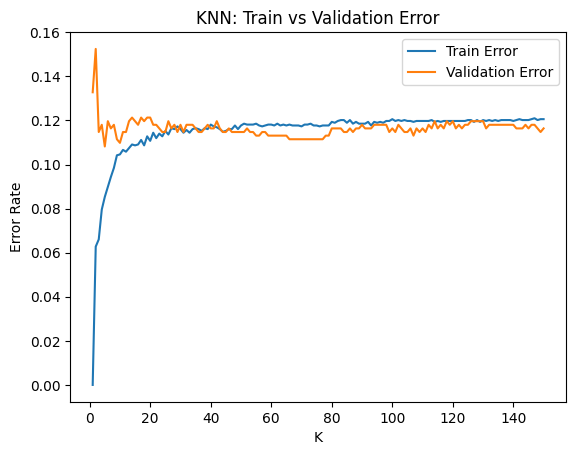
\includegraphics[width=0.65\textwidth]{knn_train_v_validation.png}
\caption{Training and Validation Error vs. K for KNN.}
\end{figure}

\noindent\textbf{(c)} Optimal $K=5$. Errors: Train 0.0853, Validation 0.1082, Test 0.1207.  

\noindent\textbf{(d)} After normalization, optimal $K=11$. Errors: Train 0.0660, Validation 0.0656, Test 0.0709.
\begin{figure}[H]
\centering
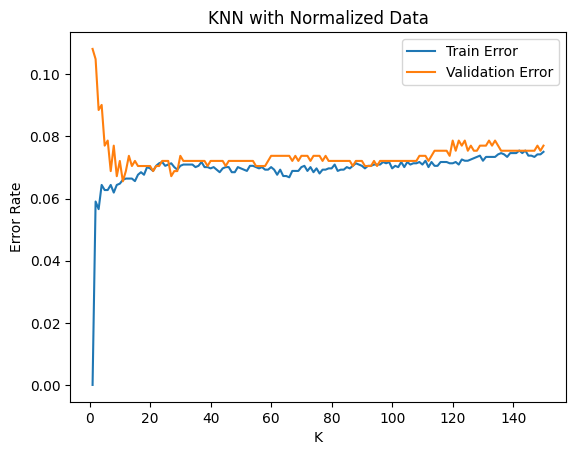
\includegraphics[width=0.65\textwidth]{knn_normalized.png}
\caption{Error vs. K for KNN with Normalized Data.}
\end{figure}

\noindent\textbf{(e)} MLP with default parameters: Train 0.0648, Validation 0.0705, Test 0.0761.  

\noindent\textbf{(f)} MLP trained with varying hidden layer sizes, shown in Figure 3.
\begin{figure}[H]
\centering
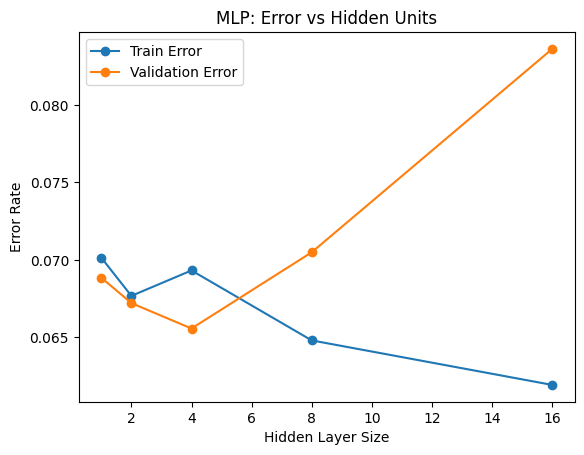
\includegraphics[width=0.65\textwidth]{mlp.png}
\caption{Error vs. Number of Hidden Units for MLP.}
\end{figure}

\noindent\textbf{(g)} Optimal hidden units = 4. Errors: Train 0.0693, Validation 0.0656, Test 0.0735. Slightly higher than KNN (0.0709).  

\noindent\textbf{(h)} Effect of changing maximum iterations in Figure 4.
\begin{figure}[H]
\centering
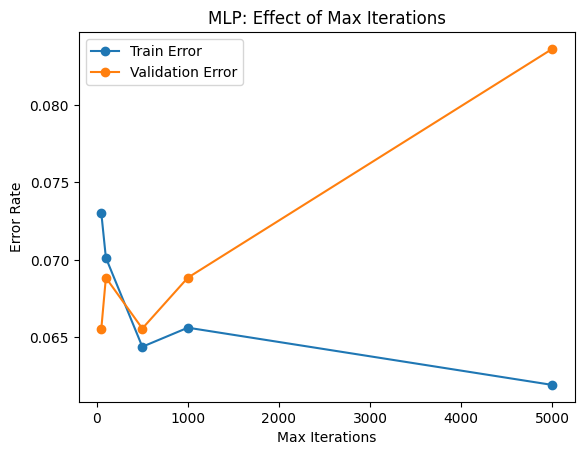
\includegraphics[width=0.65\textwidth]{mlp_max_iter.png}
\caption{Error vs. Maximum Iterations for MLP.}
\end{figure}


When training for 5000 iterations, the model begins to overfit: the training error continues to decrease while the validation error increases. Decreasing the number of iterations stops the training before the model can memorize noise in the training set, leading to better generalization and lower validation error.

This method is similar to controlling the number of hidden units when comparing the graphs. As we increase hidden units by a magnitude, the error rates are similar to what we see with higher iterations. Controlling both are valid strategies to prevent overfitting.



\noindent
\textbf{(i)} For Question 4, I utilized a generative AI assistant to help with the implementation in the `experiments.ipynb` notebook. My use of the tool was focused on improving code efficiency and formatting. I also used it for minor syntax corrections and for help in generating the plots.


\end{document}
